\documentclass{article}

\usepackage{helvet} % to change the main font
\usepackage[margin=1in]{geometry} % basically to set the margins
\usepackage{xeCJK} % to allow Chinese input
\usepackage{graphicx}
% handling the fonts and languages
\renewcommand{\familydefault}{\sfdefault}
\setCJKmainfont{FandolKai-Regular.otf}

\title{Introduction to Pattern Recognition Homework 3 Report:
Decision Trees and Random Forests}
\author{Andr\'es Ponce (彭思安)\\
\and
0616110}

\begin{document}
\maketitle


\section{Coding}
	\subsection{Gini index or Entropy is often used for meaasuring the ``best" splitting of the 
		data. Please compute the entropy and Gini Index of the provided data by the formula below.
			\[ Gini = 1 - \sum_{j}^{}p^{2}_{j}\]
			\[ Entropy = -\sum_{j}^{}p_{j}log_{2}p_{j}\]
		}
	The \textbf{Gini index} and \textbf{Entropy} are two criteria we sometimes use to measure the 
	purity or quality of a split on data. The Gini index tells us how mixed the classes are, and 
	we would like to choose the split that results in the lowest amount of mixing. The entropy is
	a measure of how much information we gain by making a split on a certain feature.

	For the provided dataset, we have the Gini index and entropy as:
	\[ Gini = 0.4628099173553719 \quad Entropy = 0.9456603046006402\]

	\subsection{Implement the Decision Tree algorithm CART and train the model by the given arguments,
				and print the accuracy score on the test data.}

		\subsubsection{Using criterion='gini', show the accuracy score of the test data by 
				max\_depth=3 and max\_depth = 10, respectively.}
				On the testing data, we were able to achieve the following accuracy\footnote{These tests used 'gini' as their purity function}:

				\begin{center} 
					\begin{tabular}{|c |c |c |}
						\hline
							clf\_depth3 & 0.9812206572769953\\\hline
							clf\_depth10 & 1.0\\
						\hline
					\end{tabular}
				\end{center}

		\subsubsection{Using max\_depth=3, show the accuracy score of test data by criterion='gini' 
						and criterion='entropy'.}
				The results for use of gini and entropy on the testing data are as follows:
				\begin{center}
						\begin{tabular}{|c |c |c |}
							\hline
							clf\_gini & 0.9370629370629371\\\hline	
							clf\_entropy & 0.9370629370629371\\\hline
						\end{tabular}
				\end{center}
		\subsection{Plot the feature importance of your Decision Tree model. You can use the model
			from question 2.1, max\_depth=10. }
			By using the somewhat complicated formula given in the reference within the sample code,
			we could arrive at the following graph for feature importance of \texttt{clf\_depth10}.

			\begin{center}
			\begin{figure}
				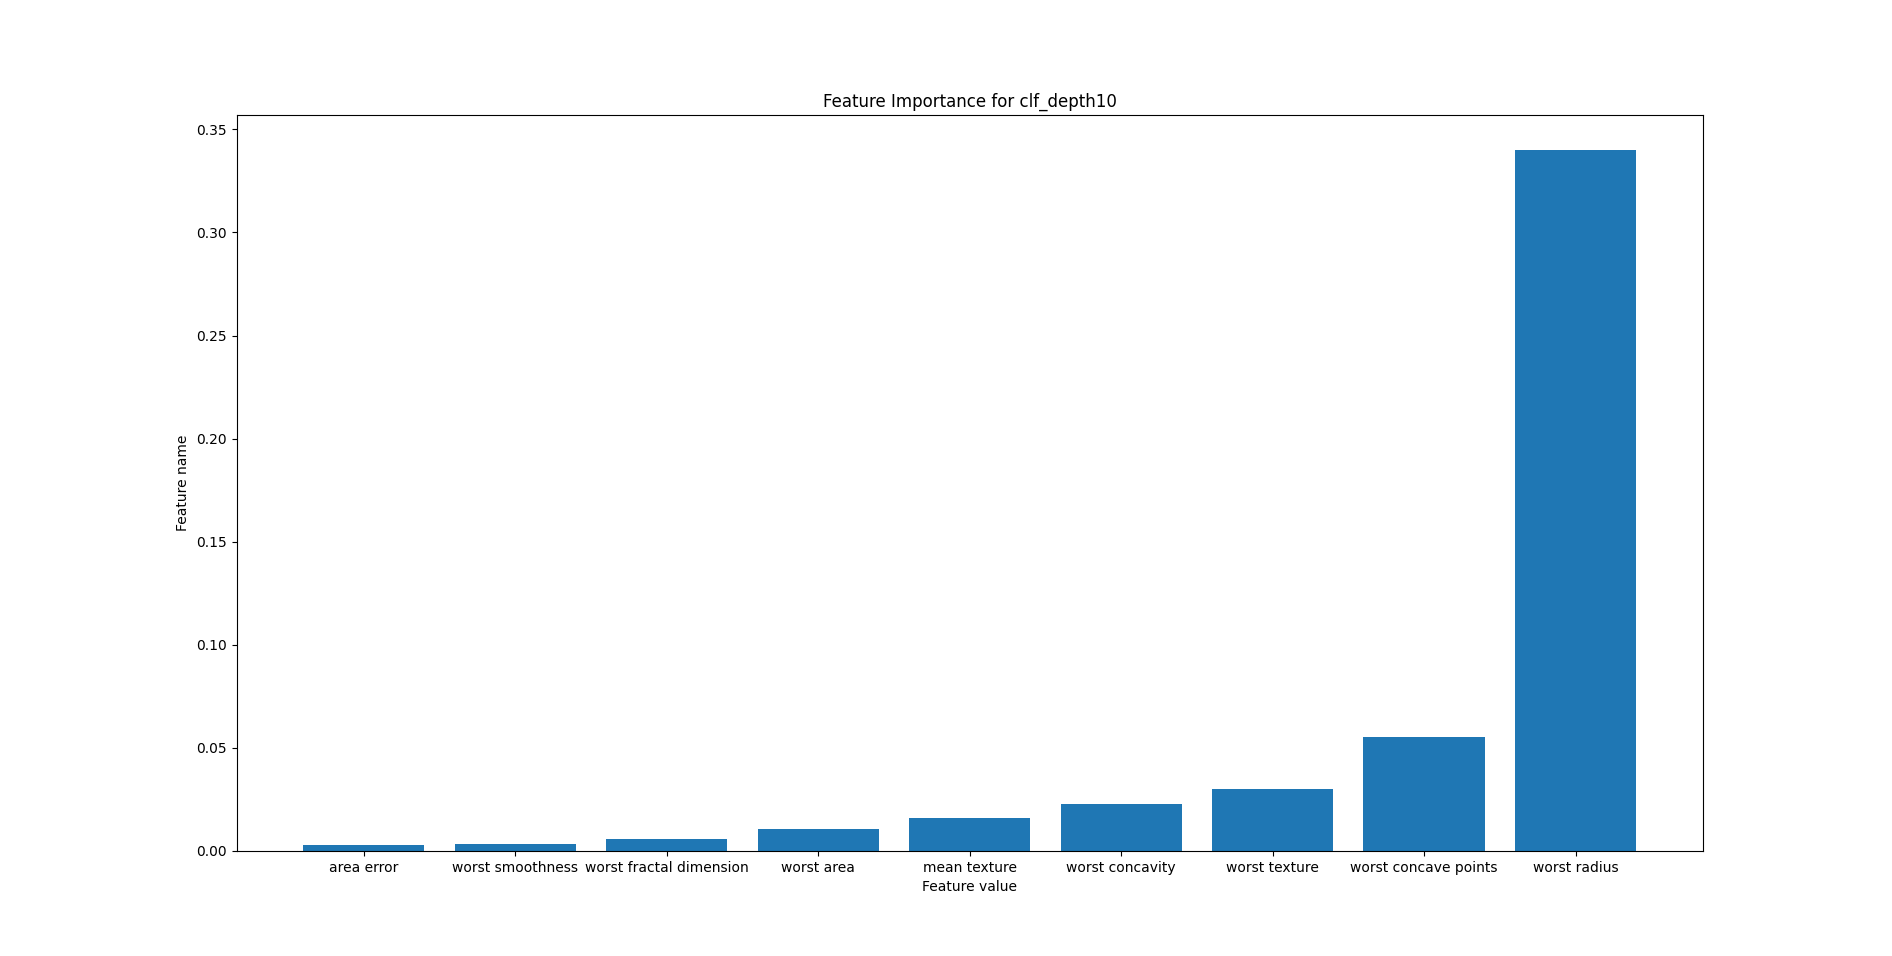
\includegraphics[scale=0.3]{Figure_1}
				\caption{Importance of the features used in tree with depth of 10.}
			\end{figure}
			\end{center}
		\subsection{Implement the Random Forest algorithm by using CART, implemented in question 2.}
			\subsubsection{Using Criterion='gini', Max\_depth=None, Max\_features=sqrt(n\_features), 
			Bootstrap=True, show the accuracy score of test data by n\_estimators = 10.}

			Using \texttt{sklearn.accuracy\_score()}, an accuracy of $1.0$ was achieved for the tree
			with Max\_depth$=10$.

			\subsubsection{Using Criterion='gini', Max\_depth=None, N\_estimators=10,Bootstrap=True,
			show the accuracy score of test data by Max\_features=sqrt(n\_features) and Max\_features
			=n\_features, respectively.}

			Again, using \texttt{sklearn.accuracy\_score()}, using Max\_Depth=None, we were able to 
			achieve approximately $0.93$ accuracy.
\section{Theory}
	\subsection{Consider a dataset comprising 400 data points from Class $C_{1}$ and 400 data points 
		from class $C_{2}$. Supose that a tree model A splits these into (300, 100) at the first leaf
		node and (100,300) at the second leaf node, where $(n,m)$ denotes that n points are assigned 
		to $C_{1}$ and m points are assigned to $C_{2}$. Similarly, suppose that a second tree model $B$
		splits them into (200, 400) and (200, 0). Evaluate the misclassification rate for the two trees
		and hence show that they are equal.}
		
		The misclassification rate involves calculating how often elements are misclassified. Therefore, 
		if we still classify the two classes into sets containing 400 elements each, then the rate that
		at which any two elements are misclassified will be the same, barring any extra information.
	\subsection{Similarly, evaluate the cross-entropy 
		\[ Entropy = - \sum_{k = 1}^{K}p_{k}log_{2}p_{k}\]
		and the Gini index
		\[ Gini = 1 - \sum_{k = 1}^{K}p^{2}_{k}\]
		for the two trees and show that they are both lower for tree B than for tree A. Define $p_{k}$
		to be the proportion of data points in region $R$ assigned to class k, where $k = 1,...,K$.
		}
		The calculations for entropy and the Gini index for the two trees are as follows

		\begin{center}
		\begin{tabular}{|c | c | c |}
			\hline
			 & Gini & Entropy\\\hline
			Tree A & $0.25$ & 0.81\\\hline
			Tree B & $0.556$ & 0.91 \\\hline
		\end{tabular}
		\end{center}
\end{document}
